\documentclass[pdflatex,sn-basic]{sn-jnl}

\usepackage{graphicx}
\usepackage{multirow}
\usepackage{amsmath,amssymb,amsfonts}
\usepackage{amsthm}
\usepackage{mathrsfs}
\usepackage[title]{appendix}
\usepackage{xcolor}
\usepackage{textcomp}
\usepackage{manyfoot}
\usepackage{booktabs}
\usepackage{algorithm}
\usepackage{algorithmicx}
\usepackage{algpseudocode}
\usepackage{listings}
\usepackage{url}
\usepackage{bm}

\theoremstyle{plain}
\newtheorem{theorem}{Theorem}
\newtheorem{proposition}[theorem]{Proposition}
\theoremstyle{definition}
\newtheorem{definition}[theorem]{Definition}

% generated by `promptcal macros` -- do not edit
\newcommand{\SPREADPTS}{0.328}
\newcommand{\SPREADFRAC}{93.8\%}
\newcommand{\SPREADMED}{0.335}
\newcommand{\AGREE}{74.8\%}
\newcommand{\NGROUPS}{14{,}631}
\newcommand{\BIGRATIO}{12}
\newcommand{\NDETS}{5{,}693{,}221}
\newcommand{\NIMAGES}{4{,}952}
\newcommand{\DETPERIMG}{1150}
\newcommand{\BANDFRAC}{2.6\%}
\newcommand{\BANDPOS}{2.9\%}
\newcommand{\APMIN}{0.462}
\newcommand{\APMAX}{0.777}
\newcommand{\APGAP}{0.315}
\newcommand{\SCBARE}{0.658}
\newcommand{\SCART}{0.568}
\newcommand{\SCPHOTO}{0.396}
\newcommand{\SCIMG}{0.436}
\newcommand{\SCPLUR}{0.540}
\newcommand{\SPREADPOS}{0.349}
\newcommand{\NPHRS}{389}
\newcommand{\FITROWS}{1{,}500{,}000}
\newcommand{\BANDID}{0.180}
\newcommand{\BANDBSID}{0.229}
\newcommand{\BANDPHC}{0.032}
\newcommand{\BANDBS}{0.175}
\newcommand{\BANDPHCNAME}{PhC (phrase, linear, band-weighted)}
\newcommand{\BANDCAT}{0.032}
\newcommand{\BANDCATF}{0.0322}
\newcommand{\BANDPHCF}{0.0324}
\newcommand{\BANDTEMP}{0.212}
\newcommand{\BANDVEC}{0.081}
\newcommand{\BANDISO}{0.125}
\newcommand{\APISO}{0.524}
\newcommand{\APID}{0.639}
\newcommand{\BANDIDN}{0.180}
\newcommand{\FACTOR}{5.6}
\newcommand{\HELDPHC}{0.022}
\newcommand{\HELDID}{0.113}
\newcommand{\HELDPLURAL}{0.229}
\newcommand{\HELDPLURALID}{0.226}
\newcommand{\HELDVEC}{0.082}
\newcommand{\COCBARE}{0.113}
\newcommand{\HELDVECIMG}{0.014}
\newcommand{\HELDBAND}{0.058}
\newcommand{\HELDBANDPL}{0.222}
\newcommand{\HELDISO}{0.042}
\newcommand{\HELDISOAP}{0.626}
\newcommand{\BANDIDCI}{0.176--0.184}
\newcommand{\BANDPHCCI}{0.028--0.034}
\newcommand{\BANDVECCI}{0.076--0.085}
\newcommand{\BOOTN}{500}
\newcommand{\DROP}{0.148}
\newcommand{\DROPCD}{0.141--0.151}
\newcommand{\FDRPOOLID}{0.41}
\newcommand{\KEPTPOOLID}{57{,}824}
\newcommand{\FDRWCID}{0.31}
\newcommand{\KEPTWCID}{44{,}163}
\newcommand{\FDRPWID}{0.31}
\newcommand{\KEPTPWID}{59{,}442}
\newcommand{\FDRPOOLPHC}{0.38}
\newcommand{\KEPTPOOLPHC}{62{,}068}
\newcommand{\FDRWCPHC}{0.29}
\newcommand{\KEPTWCPHC}{49{,}084}
\newcommand{\FDRPWPHC}{0.31}
\newcommand{\KEPTPWPHC}{61{,}087}
\newcommand{\FDRPOOLVEC}{0.39}
\newcommand{\KEPTPOOLVEC}{59{,}848}
\newcommand{\FDRWCVEC}{0.32}
\newcommand{\KEPTWCVEC}{48{,}701}
\newcommand{\FDRPWVEC}{0.32}
\newcommand{\KEPTPWVEC}{61{,}536}
\newcommand{\FDRPOOLTEMP}{0.41}
\newcommand{\KEPTPOOLTEMP}{57{,}824}
\newcommand{\FDRWCTEMP}{0.31}
\newcommand{\KEPTWCTEMP}{44{,}163}
\newcommand{\FDRPWTEMP}{0.31}
\newcommand{\KEPTPWTEMP}{59{,}442}
\newcommand{\ALPHAMAIN}{0.30}
\newcommand{\ALPHAPCT}{30\%}
\newcommand{\FDRWORST}{41\%}
\newcommand{\FDROVERSHOOT}{1.4}
\newcommand{\WCOVERSHOOT}{1.03}
\newcommand{\WCCOSTID}{24\%}
\newcommand{\WCCOSTPHC}{21\%}
\newcommand{\WCGAIN}{11\%}
\newcommand{\WCTOTALID}{44{,}163}
\newcommand{\WCTOTALPHC}{49{,}084}
\newcommand{\WCGAINFIVE}{8\%}
\newcommand{\WCKEPTFIVEID}{11{,}183}
\newcommand{\WCKEPTFIVEPHC}{12{,}131}
\newcommand{\NLVISNDET}{6{,}056{,}596}
\newcommand{\NLVISIMG}{4{,}752}
\newcommand{\NLVISCAT}{1{,}203}
\newcommand{\TRBANDID}{0.198}
\newcommand{\TRBANDPHC}{0.084}
\newcommand{\TRBANDVEC}{0.277}
\newcommand{\TRBANDTEMP}{0.243}
\newcommand{\TRBANDISO}{0.112}
\newcommand{\TRAPISO}{0.509}
\newcommand{\TRAPID}{0.577}
\newcommand{\TRAPPHC}{0.577}
\newcommand{\VECSEEN}{80}
\newcommand{\TRFACTOR}{2.4}
\newcommand{\TRAPLO}{0.409}
\newcommand{\TRAPLOID}{photo}
\newcommand{\TRAPHI}{0.710}
\newcommand{\TRAPHIID}{bare}
\newcommand{\TRAPGAP}{0.301}
\newcommand{\TRBAREID}{0.247}
\newcommand{\TRBAREPHC}{0.200}
\newcommand{\TRARTID}{0.295}
\newcommand{\TRARTPHC}{0.076}


% sn-jnl sets a 372x553pt text block, which is the block for Springer's 155x235mm trim
% size, and then lays it out on an A4 page from the top. On A4 that leaves about 75mm of
% white at the foot of every page: a fifth of the paper, and a reviewer reads it as a
% broken layout. The width is left alone -- figures and tables are cut to it -- and the
% height is extended so that the top and bottom margins are the same 76pt.
\setlength{\textheight}{690pt}
\raggedbottom

% sn-jnl caps a page at three floats. The paper has five tables and three figures and
% several of them are consecutive in the source; a cap of five costs nothing and stops a
% queue of floats from forcing a premature page break.
\setcounter{totalnumber}{5}

% sn-jnl appends ";\ " after every e-mail address, which is right for a list and leaves a
% dangling semicolon on a single-author paper.  There is one author here, so nothing follows
% the address and the separator is dropped.
\makeatletter
\def\email#1{\global\advance\emailcnt by 1\relax
  \g@addto@macro\corrauthemail{\textcolor{blue}{#1}}}
\makeatother

\begin{document}

\title[Naming the object]{Naming the object changes the answer: calibration and risk
control for open-vocabulary detectors}

\author*[1]{\fnm{Meng} \sur{Tan}}\email{mengtanmtan@gmail.com}

\affil[1]{\orgdiv{School of Computing and Artificial Intelligence}, \orgname{Southwestern University of Finance and Economics}, \orgaddress{\city{Chengdu}, \postcode{611130}, \state{Sichuan}, \country{China}}}

\abstract{An open-vocabulary detector is asked for a category by typing a phrase. The
score it returns is read as the probability that the box is right, but the score is computed
against the phrase, so it depends on the wording as much as on the region. We measure this
dependence. Holding images, boxes and categories fixed and changing only the phrasing, the
score of the same object moves by \SPREADPTS{} on average, \SPREADFRAC{} of the instances
move by more than $0.1$, and average precision ranges from \APMIN{} to \APMAX. We propose
prompt-conditioned calibration (PhC), which predicts the two parameters of an
affine-in-logit map from a 33-dimensional descriptor of the phrase, built from the text
embedding that the detector already computes. For a fixed phrase the map is strictly
increasing in the score, so average precision is unchanged, and no additional forward pass
is needed. Inside the score range where reviewers work, the calibration error falls from
\BANDID{} to \BANDPHC{} on COCO and from \TRBANDID{} to \TRBANDPHC{} on LVIS without
refitting, where a per-category table has nothing to look up. Calibration, however, is not
risk control. A threshold fitted on the mixed wordings reaches \FDROVERSHOOT{} times its
false discovery target on the wording for which it was not tuned, and no monotone map can
correct this, because the target is set by the ordering of the boxes. Selecting the
threshold within every wording does hold the target, and under that guarantee the calibrated
score keeps \WCGAIN{} more boxes than the uncalibrated one.}

\keywords{open-vocabulary detection, calibration, prompt sensitivity, conformal
selection, false discovery rate, reliability}

\maketitle

\section{Introduction}\label{sec:intro}

Open-vocabulary detectors are now used as annotation tools. A user names a category,
the detector draws boxes, and the user keeps some of them. The interface rests on a
number: the score attached to each box. Above a threshold the box is kept, below it the
box is discarded, and the value of the threshold is chosen once, from experience or from
a small labelled sample, and then reused for every category and every query.

That reuse assumes the score means the same thing across queries. For a detector driven
by a text prompt it does not, because the score is not a function of the image region
alone. The classification head compares an object query with the token embeddings of the
phrase, and the phrase is part of the input. Writing ``dog'' and writing ``a photo of a
dog'' are two different requests to the same model, and a model is free to answer them
with different confidences, different numbers of boxes, and occasionally different boxes.
Nothing in the architecture ties the two requests together.

That wording matters for accuracy is by now well documented elsewhere. In language models
the format and the order of a prompt move benchmark scores by amounts comparable to the gaps
between models \citep{sclar2024quantifying,lu2022fantastically}, and a prompt can work as well
when its content is deliberately misleading as when it is careful
\citep{webson2022prompts}; in vision--language models the template moves downstream accuracy
enough that prompts are learned rather than written \citep{zhou2022learning}. Those results are
about a dataset-level average in a classification task with a fixed label set. The question
they leave open is what the same variability means for a score that a person reads as a
probability, one box at a time, and for the threshold that score is compared against.

This paper measures that dependence and then puts it to work. Our starting point is a
public open-vocabulary detector \citep{liu2024grounding} evaluated on COCO
\citep{lin2014microsoft} and LVIS \citep{gupta2019lvis}. For every image we query the
categories that are actually present, five times, with five phrasings that a person might
type: the bare name, the name with an indefinite article, the two conventional
prompt-engineering templates, and the plural. The images, the categories and the
annotations are identical across the five runs; only the wording changes.

Three findings organise the paper.

\emph{The wording moves the score by a third of the scale.} For the same object, the
top-scoring box the model returns moves by \SPREADPTS{} on average between phrasings, and
\SPREADFRAC{} of objects move by more than $0.1$. The number of boxes above $0.5$ changes
by a factor of \BIGRATIO{} between the best and the worst phrasing. This is not a
second-order nuisance: the movement is more than half the width of the score interval in
which a reviewer actually makes decisions, and average precision itself ranges from
\APMIN{} to \APMAX{} across the five runs.

\emph{A scalar calibrator cannot repair it, because it never sees the phrase.} Global
temperature scaling, vector scaling and isotonic regression all map one number to another
number. Fitted on a mixture of phrasings they improve the aggregate error and leave the
operating band as bad as it was, or worse: the temperature that best fits the bulk of
low-scoring boxes sharpens exactly the scores a reviewer is looking at. Fitted on a single
phrasing and deployed on another, they are simply the wrong map.

\emph{What is needed is a map that knows the phrase, and a decision rule that knows what it
is buying.} We propose prompt-conditioned calibration (PhC), which predicts the two
parameters of an affine-in-logit map from a handful of descriptors of the phrase, including
a projection of the text embedding the detector already computed. Because the slope stays
positive, the map is strictly increasing in the score for a fixed phrase: it cannot reorder
two boxes asked about with the same wording, so average precision is unchanged by
construction, and the only thing it can move is where the scores sit between zero and one.
We then stop treating the threshold as a property of the score and treat it as a decision:
the threshold is chosen by conformalised selection so that the false discovery rate among
the boxes a user keeps is controlled at a target level. Here we report a result we did not
expect. A single threshold fitted on a mixture of wordings does \emph{not} deliver its
target: it arrives at \FDRWORST{} of the kept boxes wrong, against a target of \ALPHAPCT.
And no calibrator can repair that, PhC included, because the false discovery rate at a
shared threshold is set by the order of the boxes, which a monotone map is not allowed to
touch. What does hold is a threshold required to satisfy the constraint inside every
wording, and it is there that conditioning pays, if modestly: at the same target the
calibrated score keeps \WCGAIN{} more boxes than the uncalibrated one.

Our contributions are:

\begin{itemize}
\item a measurement of prompt-wording sensitivity as a first-class reliability property of
open-vocabulary detectors, on two corpora and five phrasings, with a per-run evaluation
protocol that keeps the five queries separate instead of pooling them;
\item prompt-conditioned calibration, a post-hoc map whose parameters are predicted from
phrase descriptors, strictly monotone within a phrasing, fitted on cached logits with no
additional forward pass, and --- unlike a map indexed by category --- deployable on
phrasings and vocabularies it was not fitted on;
\item a selective-detection procedure that turns the calibrated score into a threshold with
a false-discovery guarantee, and the finding --- negative for calibration, positive for
selection --- that the guarantee survives a change of wording only when the threshold is
required to hold inside each wording, not when it is fitted on the mixture;
\item a transfer study from COCO to LVIS without refitting, which separates what is a
property of the phrasing from what is a property of the corpus.
\end{itemize}

Section~\ref{sec:related} positions the work. Section~\ref{sec:task} defines the
measurement. Section~\ref{sec:method} gives the calibrator and the selection rule, and
Section~\ref{sec:exp} reports the experiments. Section~\ref{sec:discussion} discusses what
the numbers do and do not license.

\section{Related work}\label{sec:related}

\subsection{Open-vocabulary detection}

Open-vocabulary detection replaces a fixed classifier with a query: a category is described
at inference time and the detector scores regions against that description. The two families
that matter here differ in what the query is made of. Region--text alignment methods score a
region against a word embedding learned from image--caption data, either by contrasting
whole images with sentences and transferring the classifier to regions
\citep{radford2021learning} or by supervising the region--phrase alignment directly
\citep{zhong2022regionclip,yao2022detclip,minderer2023scaling}. Grounded detectors instead
fuse text tokens with image features inside the detection head, so that the classification
logit of an object query is computed against the token embeddings of the phrase. The
transformer decoder that made this possible was designed for closed-set detection
\citep{carion2020end}; MDETR conditioned it on a whole sentence \citep{kamath2021mdetr}, GLIP
recast detection as phrase grounding and scaled the grounding supervision
\citep{li2022grounded}, Grounding DINO added a cross-modality fusion stage to a DINO-style
detector \citep{liu2024grounding}, and YOLO-World and OV-DINO reorganised the same interface
for real-time inference and for a unified language-aware fusion
\citep{cheng2024yolo,wang2024ovdino}. A parallel line lets the query contain boxes as well as
words, in the form of exemplars drawn on the image
\citep{xu2023multi,jiang2023trex,jiang2024trex2}, and segmentation at any granularity shares
the interface \citep{li2024segment}. In every one of these designs the score that the
user reads is a similarity between a region and a representation of the \emph{query}, not a
posterior over a fixed label set. That is the property the rest of this paper turns on.

The literature on the query has concentrated on accuracy: which prompt template gives the
best average precision, whether prompt tuning helps \citep{zhou2022learning}, how to ensemble
prompt embeddings \citep{radford2021learning}, how to fold the vocabulary into the weights so
that a text encoder is not needed at inference time \citep{cheng2024yolo}. The question we
ask is different, and orthogonal to all of them: given that the score is a function of the
wording, what happens to the \emph{meaning} of the score when the wording changes, and what
does a threshold fitted under one wording mean under another?

\subsection{What a detection score is a probability of}

That a detector's score is not a probability is not a new observation.
\citet{hall2020probabilistic} define probabilistic object detection as the task of reporting a
detection together with its spatial and semantic uncertainty, propose an evaluation measure
without arbitrary score thresholds, and find that conventional detectors are spatially
overconfident. Monte Carlo dropout has been used in the same spirit to extract label
uncertainty from a detector and to reject objects from outside the training set
\citep{miller2018dropout}. Both treat the label as given: the uncertainty is over \emph{where}
the object is and \emph{which} of the known classes it belongs to, and the quantity that is
miscalibrated is a property of the image and the network. Once the label is a sentence typed
at inference time, the object of uncertainty changes. The same region scored against
\emph{dog} and against \emph{a photo of a dog} is two different queries, and the two scores are
two different claims about the same pixels. This paper is about the second kind of
variability, which the probabilistic detection literature does not have to consider because
its label set is fixed.

\subsection{Calibration of detectors}

Post-hoc calibration maps a score to a probability using held-out data. The classical options
are parametric, Platt scaling \citep{platt1999probabilistic} and its per-group generalisation,
and non-parametric, histogram binning and isotonic regression \citep{zadrozny2002transforming};
temperature scaling \citep{guo2017calibration} is the one-parameter version that leaves
accuracy untouched because it is monotone. Calibrated regression
\citep{kuleshov2018accurate} generalises the idea to continuous outputs, and a body of work
examines when and how these estimators fail
\citep{vaicenavicius2019evaluating,nixon2019measuring,wang2023calibration}.

Two assumptions of that literature are violated in our setting. First, calibration is usually
evaluated as an average over the whole score range, which for a detector is dominated by the
boxes nobody keeps; we therefore report the error inside the band where review actually
happens. Second, and more importantly for this paper, the calibrated object is assumed to be
the model's output on a fixed input distribution. When the input includes a user-typed phrase,
the distribution that matters is indexed by the phrase, and a map fitted on the marginal over
phrasings is not the right map for any of them.

The closest precedent lives in a different modality, and it is close enough that the
difference is worth stating precisely. \citet{zhao2021calibrate} observed that the few-shot
accuracy of a language model swings with the prompt format and traced the swing to a bias
towards particular answers; they estimate that bias with a content-free input such as
``N/A'' and fit, per prompt, an affine map that makes the content-free prediction uniform.
The premise --- that the object to calibrate is the pair (model, prompt) rather than the model
alone --- is the one we adopt, and the affine form is the same. What differs is how the map is
obtained and what it is asked to deliver. A detector has no content-free input: there is no
image whose detection scores would reveal the bias of the phrase \emph{a photo of a}, so the
map cannot be measured at deployment from unlabelled probes and has to be predicted from the
phrase itself. And the target here is not an aggregate accuracy but the calibration of
individual detections inside an operating band, together with the ordering that a threshold
acts on. Section~\ref{sec:exp-fdr} shows that the second of these is out of reach for
any recalibration, contextual or otherwise, which is why the phrase-conditioned map is only
half of our proposal and the threshold protocol is the other half.

\subsection{Conformal selection and risk control}

Turning a score into a decision with a guarantee is a separate problem from making the score a
probability. Selective prediction trades coverage for accuracy
\citep{geifman2017selective,geifman2019selectivenet}, and conformal prediction supplies
distribution-free coverage guarantees \citep{angelopoulos2023conformal}. Risk-controlling
prediction sets \citep{bates2021distribution} generalise the guarantee from coverage to an
arbitrary monotone loss calibrated on a holdout set, and conformalised selection
\citep{jin2023selection} is the false-discovery-rate case of that framework, which is the
quantity a user of a detection tool cares about: of the boxes I keep, what fraction is wrong.
The procedure needs a labelled calibration sample and an exchangeability assumption between
calibration and test. In a deployment where the user types an arbitrary phrase,
exchangeability holds comfortably within a phrasing and not at all across phrasings. We adopt
the procedure and then test that assumption directly, and the answer is negative: a threshold
fitted on a mixture of wordings does not deliver its target on the wordings the mixture
contains, and no monotone recalibration of the score changes that, because the target depends
on the ordering of the boxes rather than on the scale. Requiring the constraint to hold
\emph{inside} each wording does deliver it, at a cost in kept boxes that is smaller when the
scores of the wordings already agree --- which is the sense in which conditioning the phrase
pays for itself.

\subsection{Sensitivity to the prompt}

That a prompt's wording moves the output is by now well documented, mostly for language
models. The \emph{format} of a prompt alone --- separators, casing, spacing --- produces
accuracy spreads comparable to the differences between models, and the spread is stable
enough to be measured by a sensitivity metric computed over a set of format variations
\citep{sclar2024quantifying}. The \emph{order} of few-shot examples does the same: some
permutations are near state of the art and others near chance, and a good permutation for one
model does not transfer to another \citep{lu2022fantastically}. A stronger result is that many
intentionally irrelevant or even misleading prompts work as well as carefully written ones,
which undermines the reading that a prompt is understood as an instruction
\citep{webson2022prompts}. On the vision--language side the template matters enough that a
prompt is learned rather than written \citep{zhou2022learning}, and CLIP already ensembles
several hand-written templates because no single one is best \citep{radford2021learning}.

All of this work measures the effect on accuracy: a dataset-level scalar, in a classification
task where the label set is fixed and every input has one correct answer. The effect we study
is of the same origin --- the wording is arbitrary from the model's point of view, which is
the lesson of \citet{webson2022prompts} --- but it is measured somewhere else. We measure it on
the probability assigned to an \emph{individual detection}, and the quantity at stake is not
accuracy but the meaning of a threshold: a detector whose average precision barely moves can
still have an operating point that means something entirely different under a different
sentence, and that is the case a deployment notices.

\subsection{What is new here}

Calibration, conformal selection and prompt sensitivity are mature as separate literatures,
and the idea of calibrating per prompt exists in another modality. To our knowledge this is
the first study that (i) measures the phrasing-induced shift as a property of the individual
detection rather than of the dataset-level average precision, (ii) predicts a calibrator's
parameters from the phrase representation, so that a wording not seen during fitting is
calibrated without a deployment-time probe, (iii) separates what calibration can buy from
what it cannot --- it moves the scale, so it repairs the band, and it cannot move the ordering,
so it cannot rescue a shared threshold --- and locates the coverage gain of a
phrase-conditioned score in the threshold-selection protocol rather than in the calibrator
alone, and (iv) evaluates the five wordings as five separate runs instead of pooling them,
which is what a deployment actually sees.

\section{Measuring the dependence on wording}\label{sec:task}

\subsection{What is held fixed}

We evaluate on COCO val2017 \citep{lin2014microsoft}, 5{,}000 images of which \NIMAGES{}
carry annotations, over 80 categories, and on the LVIS v1.0 minival split
\citep{gupta2019lvis}, 4{,}809 images and 1{,}203 categories; LVIS images are the same COCO 2017 JPEGs, so the two corpora share a pixel
source and differ in annotations and vocabulary.

The detector is Grounding DINO \citep{liu2024grounding} with the public Swin-T checkpoint.
It is used exactly as distributed: no fine-tuning, no prompt tuning, no threshold tuning.
For each image we query the categories that are actually annotated in it, which is the
realistic case for an annotation assistant (a user points at what is there) and avoids
inflating the false-positive count with categories that were never asked for.

Each image is queried five times. In the $v$-th run the phrase for category $c$ is

\begin{equation}
\phi_v(c) = \big(\text{name},\ \text{a name},\ \text{a photo of a name},\
\text{an image of a name},\ \text{names}\big)_v ,
\end{equation}

that is: the bare name, an indefinite article, the two templates that circulate as prompt
engineering for region--text models, and the plural. We call these the five \emph{wordings}
and write $\phi$ for a phrase. Everything else, including the image, the category, the
post-processing and the weights, is identical across the five runs, so any difference in
the output is attributable to the phrase.

\subsection{Detection records}

Within a run, detections are kept at a score threshold of $0.01$ and capped at the top 80
per (image, category) pair, which is well inside the operating range of the detector and
leaves \NDETS{} records on COCO. A detection is \emph{correct} if it matches a
ground-truth instance of the queried category at IoU $\geq 0.5$, assigned greedily in
descending score. Matching is done separately inside each run: the five runs are five
queries, and letting them share one ground-truth instance would score four of the five as
wrong by construction.

Table~\ref{tab:setup} summarises the two corpora. The band $p\in[0.3,0.9)$ is where a human
reviews boxes: it is \BANDFRAC{} of the output of a run and holds \BANDPOS{} of its true
positives, and it is where the detector is least reliable, with a band error of
\BANDIDN.

\begin{table}[t]
\caption{The five wordings on the same images with the same weights. A row is one phrasing; nothing but the text query changes between rows. ``Band'' is $p\in[0.3,0.9)$ of the uncalibrated score.}
\label{tab:setup}
\begin{tabular*}{\textwidth}{@{\extracolsep{\fill}}lrrrrrr@{}}
\toprule
Wording & detections & per image & positive rate & AP & share in band & ECE \\
\midrule
bare               & 1{,}063{,}949 & 215 & 3.2\% & 0.7770 & 4.3\% & 0.0500 \\
article            & 1{,}155{,}657 & 233 & 2.8\% & 0.7430 & 2.0\% & 0.0602 \\
photo              & 1{,}170{,}394 & 236 & 2.6\% & 0.4622 & 1.9\% & 0.0596 \\
image              & 1{,}169{,}850 & 236 & 2.7\% & 0.5020 & 2.2\% & 0.0512 \\
plural             & 1{,}133{,}371 & 229 & 3.0\% & 0.7217 & 2.6\% & 0.0474 \\
\bottomrule
\end{tabular*}
\end{table}


\subsection{Metrics, and why they are computed per run}

The five runs are evaluated separately and the results averaged; pooling them would let one
phrasing contribute five copies of the same ground-truth instance and would hide exactly the
effect we are measuring. Inside a run we report:

\begin{itemize}
\item the expected calibration error over 15 bins (ECE), and the same quantity restricted to
the operating band with 10 bins (band ECE);
\item the Brier score, a proper score, and its restriction to the band (band Brier). The
restricted Brier is the quantity we trust most: it needs no binning, and on the band it is
computed on the boxes a reviewer would actually see;
\item average precision (AP) at 101 recall points, computed per category, and the area under
the risk--coverage curve (AURC) for the selective-prediction view.
\end{itemize}

AP here is not the official benchmark metric and is not comparable to published
zero-shot numbers: matching happens inside a run and only over the categories that were
asked for, so there is no penalty for the categories the image does not contain. It is
used only to compare the five runs, and the calibrators within a run, on identical
candidates.

The band mask of a run is fixed by that run's \emph{uncalibrated} score, so every calibrator
is scored on the same detections. Calibrators are fitted on one half of the images and
evaluated on the other, split by image rather than by detection: one image contributes about
\DETPERIMG{} queries that are strongly correlated, and a detection-level split would place
near-copies on both sides.

\subsection{The quantity we are after}

For an object, we take the highest-scoring box the detector returns for its category in each
of the five runs. If the phrasing did not matter, these five numbers would agree. We report
their range, the fraction of objects whose range exceeds $0.1$, and how often the five runs
disagree about whether the box is correct at all. The same object, five scores, is the unit
of the measurement; Section~\ref{sec:exp-measure} reports it.

\section{Method}\label{sec:method}

\subsection{Prompt-conditioned calibration}

Let $z$ be the raw classification logit of a detection and $\phi$ the phrase that was used to
request its category. A scalar calibrator fits one map $z\mapsto\sigma(az+b)$ for all
detections. We instead let the two parameters be functions of the phrase:

\begin{equation}\label{eq:phc}
p = \sigma\!\left(z\,e^{-\ell(\phi)} + m(\phi)\right),
\qquad
\ell(\phi) = \log T(\phi),\quad m(\phi) = b(\phi),
\end{equation}

where $\ell$ and $m$ are produced by a linear head on a descriptor $x(\phi)$ of the phrase.
Since $T(\phi)=e^{\ell(\phi)}>0$ for every phrase, the map is strictly increasing in $z$ for
fixed $\phi$.

\begin{proposition}[The map cannot reorder a run]\label{prop:mono}
For any two detections that were requested with the same phrase, $z_i>z_j$ implies
$p_i>p_j$ under \eqref{eq:phc}. Consequently every ranking metric computed within a
single-wording run, including average precision and the risk--coverage curve, is unchanged by
the calibrator.
\end{proposition}

\begin{proof}
$T(\phi)>0$, so $z\mapsto z/T(\phi)+m(\phi)$ is strictly increasing, and $\sigma$ is strictly
increasing.
\end{proof}

This property is what makes the method safe to use. The map can change the score scale, which
is what thresholds and calibration error are about, and it cannot change the order of the boxes
that a user sees in one run, which is what AP is about. A map that may depend on $z$ in a
non-monotone way, such as isotonic regression, does not have this property, and
Table~\ref{tab:main} reports the AP that it costs.

\paragraph{The phrase descriptor.} $x(\phi)$ has 33 entries. The first 24 are a principal
component projection of the pooled last-layer text embedding that the detector's own text
encoder produced for $\phi$, averaged over tokens. This requires no extra forward pass, because
the encoder has already run. The remaining entries are the token count, the character length,
the embedding norm, the cosine similarity to the bare name of the same category, and a one-hot
encoding of the five wordings. The head is linear, so the whole calibrator has 68 parameters. We
use a linear head because the calibrator has to be fitted on the phrases that one is willing to
enumerate, and a linear map on interpretable descriptors degrades gracefully when the deployed
phrase lies outside that set.

\paragraph{Fitting.} The parameters minimise a weighted Brier loss on cached logits,
\begin{equation}
\mathcal{L} = \frac{1}{n}\sum_i w_i\,\big(p_i - y_i\big)^2 ,
\qquad
w_i = \begin{cases} w_{\rm band} & \text{if the uncalibrated score is in the band}\\ 1 & \text{otherwise,}\end{cases}
\end{equation}
with $w_{\rm band}=10$ in the default configuration. The band is computed once from the
uncalibrated score and then frozen. If it were recomputed from the output of the model, the
cheapest way to lower a band-weighted loss would be to push boxes out of the band rather than to
calibrate them.

\subsection{From a calibrated score to a threshold}

A calibrated probability is not yet a decision. The user of an annotation tool sets a threshold
$\lambda$ and keeps every box with $p\geq\lambda$. What the user cares about is the false
discovery rate among the kept boxes, $\mathrm{FDR}=\mathbb{E}[V/R]$, where $R$ is the number
kept and $V$ is the number of these that are wrong.

We choose $\lambda$ on a labelled calibration half by conformalised selection
\citep{jin2023selection}. The calibration detections are ordered by decreasing score. Let $R(k)$
and $V(k)$ be the number kept and the number wrong among the top $k$, and set

\begin{equation}\label{eq:lambda}
\hat\lambda = \min\Big\{\lambda \;:\; \frac{1+V(\lambda)}{\max(R(\lambda),1)} \leq \alpha\Big\},
\end{equation}

the smallest threshold whose conformal estimate of the false discovery proportion is below the
target $\alpha$. Under exchangeability of calibration and test detections this controls
$\mathbb{E}[\mathrm{FDR}]$ at $\alpha$ up to a term of order $1/R$
\citep{jin2023selection,angelopoulos2023conformal}.

The exchangeability assumption is the part that matters here. It holds comfortably when the
calibration and the test detections come from the same phrasing, and it fails when they do not.
A threshold calibrated on ``dog'' and applied to ``dogs'' is not covered by the theorem, and
Section~\ref{sec:exp-fdr} measures how far it misses.

One might expect that conditioning the score on the phrase restores the assumption, by making
detections requested with different wordings comparable. It does not, and
Proposition~\ref{prop:mono} shows why. The false discovery rate at a shared threshold is a
function of the \emph{order} of the kept boxes, and a monotone map leaves that order untouched.
If two wordings disagree about which boxes are the good ones, calibration cannot reconcile
them. What does work is to require the constraint within each wording:

\begin{equation}\label{eq:lambda-worst}
\hat\lambda_{\max}(\alpha) \;=\; \max_{v\in\{1..5\}} \hat\lambda_v(\alpha),
\end{equation}

where $\hat\lambda_v$ is \eqref{eq:lambda} computed on the calibration detections of wording $v$
alone. Since $\mathrm{FDR}$ falls as the threshold rises, \eqref{eq:lambda-worst} is the
strictest admissible choice, and it satisfies the constraint in every wording at the same time.
Because it is a maximum over strata, it needs no multiplicity correction. It is also the only one
of the three threshold protocols compared in Table~\ref{tab:fdr} that a tool can deploy as a
single number and still satisfy the constraint in every wording. Section~\ref{sec:exp-fdr}
reports what it costs.

\begin{table}[t]
\caption{The three protocols compared for every calibrator. A run is one phrasing on all
images. ``Mixed'' fits on all five wordings; ``held-out'' fits on three and is applied to the
two it never saw; ``transfer'' fits on COCO and is applied to LVIS.}\label{tab:protocols}
\begin{tabular*}{\textwidth}{@{\extracolsep{\fill}}lll@{}}
\toprule
Protocol & Fitted on & Evaluated on \\
\midrule
mixed & five wordings, half the images & the other half, all five \\
held-out wording & bare, article, photo & image, plural \\
transfer & COCO, five wordings & LVIS, five wordings, no refit \\
\bottomrule
\end{tabular*}
\end{table}

\section{Experiments}\label{sec:exp}

\subsection{What is measured, and on what}

The detector is Grounding DINO \citep{liu2024grounding} with the public Swin-T
checkpoint, used exactly as distributed. Every image is queried with the phrases of the
categories that are annotated in it, once per wording, so that the five runs of an image
differ in nothing but the text. COCO contributes \NIMAGES{} images and 80 categories, which
the five wordings turn into \NPHRS{} distinct query phrases; the extraction takes about a
second per image for all five runs together, which is the cost of the measurement rather
than of the method.

A calibrator sees only cached \emph{(logit, phrase, label)} triples: it never touches an
image and never runs the detector. PhC accordingly fits on \FITROWS{} rows in seconds, and
adds 68 parameters to a 172\,M-parameter model.

\subsection{The wording moves the score}\label{sec:exp-measure}

Table~\ref{tab:setup} and Fig.~\ref{fig:word} report the measurement of
Section~\ref{sec:task}. The five rows are the same images, the same weights, the same
post-processing and the same category; the only difference is the sentence the user typed.

\begin{table}[t]
\caption{The five wordings on the same images with the same weights. A row is one phrasing; nothing but the text query changes between rows. ``Band'' is $p\in[0.3,0.9)$ of the uncalibrated score.}
\label{tab:setup}
\begin{tabular*}{\textwidth}{@{\extracolsep{\fill}}lrrrrrr@{}}
\toprule
Wording & detections & per image & positive rate & AP & share in band & ECE \\
\midrule
bare               & 1{,}063{,}949 & 215 & 3.2\% & 0.7770 & 4.3\% & 0.0500 \\
article            & 1{,}155{,}657 & 233 & 2.8\% & 0.7430 & 2.0\% & 0.0602 \\
photo              & 1{,}170{,}394 & 236 & 2.6\% & 0.4622 & 1.9\% & 0.0596 \\
image              & 1{,}169{,}850 & 236 & 2.7\% & 0.5020 & 2.2\% & 0.0512 \\
plural             & 1{,}133{,}371 & 229 & 3.0\% & 0.7217 & 2.6\% & 0.0474 \\
\bottomrule
\end{tabular*}
\end{table}


\begin{figure}[t]
\centering
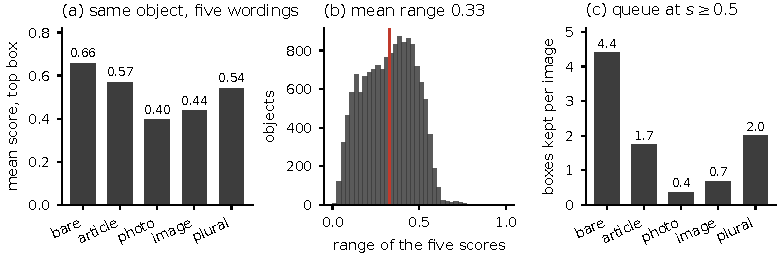
\includegraphics[width=\textwidth]{fig/fig1_wording.pdf}
\caption{The same objects, five wordings. (a) Mean score of the box the detector is most
confident about for an object, per wording. (b) Distribution over \NGROUPS{} objects of the
range of those five scores; the line is the mean. (c) How many boxes survive a fixed score cut of $0.5$, per
image: the queue a reviewer would be handed under a default threshold.}
\label{fig:word}
\end{figure}

Two sentences that name the same category do not produce the same number. The mean score
of the top box for an object is \SCBARE{} under the bare name, \SCART{} with an article,
\SCPHOTO{} under ``a photo of a'', \SCIMG{} under ``an image of a'' and \SCPLUR{} in the
plural: the five averages span a quarter of the scale, and the range within an object
(\SPREADPTS{} below) is wider still. Per object the range
of the five scores averages \SPREADPTS{} (median \SPREADMED), exceeds $0.1$ for \SPREADFRAC{}
of the \NGROUPS{} objects we can measure, and is \SPREADPOS{} even on the objects that all
five runs get right, where by construction there is nothing but the score to disagree
about. The disagreement is not confined to the score: the five runs agree on whether the
top box is correct at all for only \AGREE{} of the objects.

The consequence at a fixed threshold is immediate. A default cut of $0.5$ keeps
\BIGRATIO{} times as many boxes under one wording as under another
(Fig.~\ref{fig:word}c), so a reviewer who sets a threshold by eye under one phrasing has
set a different threshold under the next.

Average precision moves as well, from \APMIN{} to \APMAX{} (\APGAP). Part of that is
mechanical, because the score floor and the per-pair cap of Section~\ref{sec:task} discard
different boxes in different runs, so the five runs do not offer the same candidates. The
rest is not mechanical: among the boxes that survive, the phrasing also changes their
order, which is the part no post-hoc map can repair
(Proposition~\ref{prop:mono}). Either way the practical statement is the same one: with a
fixed capacity budget the detector returns a different amount of usable output depending
on how the user phrased the request.

\subsection{Calibrating the band}\label{sec:exp-calib}

Table~\ref{tab:main} fits each calibrator on half the images and evaluates on the other
half, inside each wording run, and averages over the five runs.

\begin{table}[t]
\caption{Calibration on the COCO half the calibrator never saw. Metrics are computed inside each wording run and averaged over the five runs. ``Band'' restricts to $p\in[0.3,0.9)$ of the uncalibrated score of that run. Lower is better except AP.}
\label{tab:main}
\begin{tabular*}{\textwidth}{@{\extracolsep{\fill}}lrrrrr@{}}
\toprule
Method & band ECE & band Brier & ECE & Brier & AP \\
\midrule
uncalibrated                       & 0.1800 & 0.2287 & 0.0536 & 0.0199 & 0.6395 \\
temperature scaling                & 0.2123 & 0.2421 & 0.0087 & 0.0173 & 0.6395 \\
vector scaling                     & 0.0812 & 0.1849 & 0.0051 & 0.0158 & 0.6395 \\
isotonic regression                & 0.1246 & 0.2428 & 0.0076 & 0.0180 & 0.5236 \\
per-wording temperature            & 0.2108 & 0.2418 & 0.0079 & 0.0172 & 0.6395 \\
PhC (phrase, linear)               & 0.0597 & 0.1817 & 0.0040 & 0.0157 & 0.6395 \\
PhC (phrase, linear, band-weighted) & 0.0324 & 0.1754 & 0.0068 & 0.0157 & 0.6395 \\
PhC+category                       & \textbf{0.0322} & \textbf{0.1729} & 0.0065 & 0.0155 & 0.6395 \\
\bottomrule
\end{tabular*}
\end{table}


\begin{figure}[t]
\centering
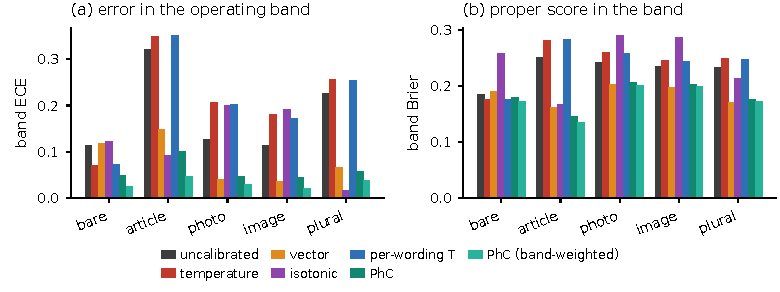
\includegraphics[width=\textwidth]{fig/fig2_calib.pdf}
\caption{Band ECE (a) and band Brier (b) per wording, for the calibrators of
Table~\ref{tab:main} except the per-category variant, on the half of COCO the calibrator did
not see. The band is fixed by the uncalibrated score of each run,
so all bars of a group are computed on the same detections.}
\label{fig:calib}
\end{figure}

Prompt-conditioned calibration reduces the error in the operating band from \BANDID{}
[\BANDIDCI] to \BANDPHC{} [\BANDPHCCI], a factor of \FACTOR, and the proper score on the same
detections from \BANDBSID{} to \BANDBS. The brackets are 95\% intervals from \BOOTN{}
resamples of the test images, which is the right unit: the rows of one image are strongly
correlated, so a detection-level interval would be far too narrow. The reduction itself is
\DROP{} [\DROPCD]. The two scalar baselines do not merely fail to help, they hurt:
temperature scaling raises the band error to \BANDTEMP{} and a separate temperature per
wording, the strongest scalar model available once the wording is known, to a level
indistinguishable from it. This is the point of Section~\ref{sec:method}: the two
parameters are fitted to an objective dominated by the $97\%$ of detections outside the
band, and the band inherits whatever is left over.

Two rows deserve comment. Vector scaling reaches \BANDVEC{} [\BANDVECCI], an interval that
does not overlap PhC's, because a per-category scale and bias absorb much of what the phrase
does --- at the price of a table indexed by category, which Section~\ref{sec:exp-transfer}
shows is exactly what does not survive a new vocabulary. Isotonic regression reaches
\BANDISO{} and pays for it with \APISO{} against \APID: it is free to reorder a run, and it
does. Every method in the table that \emph{is} monotone within a run reports the same AP as
doing nothing, \APID, which is Proposition~\ref{prop:mono} measured rather than assumed.

The last row adds a term indexed by category to PhC and is the best in both error columns, by
\BANDCATF{} against \BANDPHCF{}: a difference in the fourth decimal, well inside the interval
above. Once the descriptor of the phrase is in the map, the category table has nothing left to
supply on the corpus it was fitted on; on a corpus whose categories are new it has nothing to
look up at all (Section~\ref{sec:exp-transfer}). We therefore carry PhC without the table, and
the bold entries of Table~\ref{tab:main} are simply the minima of their columns, not the
configuration we recommend.

\subsection{A wording the calibrator has not seen}\label{sec:exp-heldout}

A practitioner can enumerate the phrasings they use; they cannot enumerate the ones their
users will type. Table~\ref{tab:heldout} therefore fits on bare, article and photo, and
deploys on ``an image of a'' and the plural, which the calibrator has never seen. The
uncalibrated row is the reference: a calibrator is only useful here if it beats doing
nothing on a wording it was not fitted on.

\begin{table}[t]
\caption{Fitted on three wordings (bare, article, photo) and deployed on the two it never saw. The uncalibrated row is the reference: a calibrator is only useful here if it beats doing nothing on an unseen wording.}
\label{tab:heldout}
\begin{tabular*}{\textwidth}{@{\extracolsep{\fill}}lrrrr@{}}
\toprule
Method & \multicolumn{2}{c}{``an image of a''} & \multicolumn{2}{c}{plural} \\
\cmidrule(lr){2-3}\cmidrule(l){4-5}
 & band ECE & band Brier & band ECE & band Brier \\
\midrule
uncalibrated                       & 0.1128 & 0.2342 & 0.2257 & 0.2333 \\
temperature scaling                & 0.1847 & 0.2472 & 0.2580 & 0.2509 \\
vector scaling                     & 0.0144 & 0.2041 & 0.0818 & 0.1802 \\
isotonic regression                & 0.2187 & 0.2975 & 0.0424 & 0.2143 \\
per-wording temperature            & 0.1873 & 0.2480 & 0.2593 & 0.2518 \\
PhC (phrase, linear)               & 0.0653 & 0.2130 & 0.2342 & 0.2378 \\
PhC (phrase, linear, band-weighted) & 0.0577 & 0.2142 & 0.2225 & 0.2360 \\
PhC+category                       & 0.0217 & 0.2023 & 0.2289 & 0.2415 \\
\bottomrule
\end{tabular*}
\end{table}


On ``an image of a'' PhC brings the band error from \HELDID{} down to \HELDBAND{} with no
category table, and to \HELDPHC{} with one. On the plural neither helps: \HELDBANDPL{} and
\HELDPLURAL{} against \HELDPLURALID{} for doing nothing.

Vector scaling is much better than any of them on both unseen wordings, \HELDVECIMG{} and
\HELDVEC{}, and the reason is instructive. Its table is indexed by category, and the
categories here are the ones it was fitted on --- only the sentence is new, so the entry
for a category still supplies the category-specific part of the offset while the shared scale
absorbs the wording. Section~\ref{sec:exp-transfer} shows the same table failing completely
when the categories are the new part. The two experiments therefore locate the difficulty on
two different axes: a per-category table generalises along wordings and not along
vocabularies, a phrase descriptor generalises along vocabularies and only partly along
wordings. PhC leads on COCO because there both axes are inside its training set; a wording it
has not seen is the case where it falls behind a table.

Isotonic regression reaches \HELDISO{} on the plural, the best number in the table, and pays
\HELDISOAP{} against \APID{} for it: it is allowed to reorder the run, which is the freedom the
other rows do not have (Proposition~\ref{prop:mono}).

We report this because it delimits the claim: PhC is not a substitute for a category table
when the categories are known and the wording is not. What it substitutes for is the category
table itself, and that is the setting in which an open-vocabulary detector is actually used.

\subsection{What a threshold is worth}\label{sec:exp-fdr}

A calibrated score is not yet a decision. Table~\ref{tab:fdr} compares three ways to end
up with a threshold at target $\alpha=\ALPHAMAIN$, and reports for each the false
discovery rate of the \emph{worst} of the five wordings, which is what a guarantee has to
cover.

\begin{table}[t]
\caption{Three ways to choose a threshold at target $\alpha=0.30$, fitted on the calibration half and measured on the other. ``Pooled'' is one $\hat\lambda$ from the calibration rows of all five wordings, ``worst-case'' is the most conservative of the five per-wording $\hat\lambda$, and ``per-wording'' selects inside each wording. Each cell pair gives the false discovery rate of the \emph{worst} of the five wordings and the number of boxes kept across all five. The worst wording is the one that a guarantee has to cover.}
\label{tab:fdr}
\begin{tabular*}{\textwidth}{@{\extracolsep{\fill}}lrrrrrr@{}}
\toprule
 & \multicolumn{2}{c}{pooled $\hat\lambda$} & \multicolumn{2}{c}{worst-case $\hat\lambda$} & \multicolumn{2}{c}{per-wording $\hat\lambda$} \\
\cmidrule(lr){2-3}\cmidrule(lr){4-5}\cmidrule(l){6-7}
Score & max FDR & kept & max FDR & kept & max FDR & kept \\
\midrule
uncalibrated & 0.406 & 57{,}824 & 0.310 & 44{,}163 & \textbf{0.310} & 59{,}442 \\
temperature scaling & 0.406 & 57{,}824 & 0.310 & 44{,}163 & \textbf{0.310} & 59{,}442 \\
vector scaling & 0.393 & 59{,}848 & 0.321 & 48{,}701 & 0.321 & 61{,}536 \\
PhC (phrase, linear) & \textbf{0.380} & 62{,}068 & \textbf{0.294} & 49{,}084 & 0.313 & 61{,}087 \\
\bottomrule
\end{tabular*}
\end{table}


\begin{figure}[t]
\centering
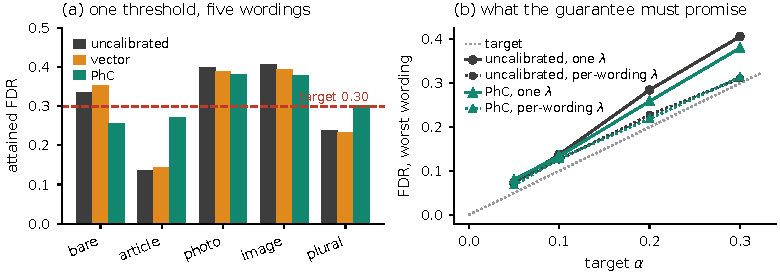
\includegraphics[width=\textwidth]{fig/fig3_fdr.pdf}
\caption{(a) False discovery rate actually attained under a single pooled threshold
calibrated at $\alpha=0.30$, per wording. (b) Attained FDR of the worst wording as the
target varies, for a single threshold and for one threshold per wording.}
\label{fig:fdr}
\end{figure}

The pooled threshold is the natural thing to ship and it does not work. Calibrated on the
mixed wordings at $\alpha=\ALPHAMAIN$, it delivers \FDRWORST{} on the wording that fares
worst --- an overshoot by a factor of \FDROVERSHOOT{} --- and Fig.~\ref{fig:fdr}a shows
the ordering of the five wordings, not a uniform bias that a better global calibration
could absorb.

The reason is Proposition~\ref{prop:mono} read backwards. The false discovery rate at a
shared threshold is set by the \emph{order} of the boxes within each run, and no monotone
map can change that order. Calibration moves the scale, so it can make scores comparable,
but it cannot make two wordings agree about which boxes are the good ones when they
already disagree. None of the five calibrators in Table~\ref{tab:main}, including PhC,
closes the gap; Fig.~\ref{fig:fdr}b shows the residual, and we report it as a negative
result because it is the one we did not expect.

What does hold is a threshold chosen to satisfy the constraint inside every wording
separately. Taking the strictest of the five per-wording thresholds needs no multiplicity
correction --- the maximum over strata is the simultaneous statement --- and its worst wording
lands at \FDRWCPHC{} for PhC and \FDRWCID{} for the uncalibrated score (Table~\ref{tab:fdr},
middle block), against a target of \ALPHAMAIN. That is an excess of one point, where the
pooled threshold is eleven points over, and it is the calibration-to-test gap of a finite
sample rather than a systematic overshoot: the threshold is fitted on one half and measured on
the other. It costs boxes, and
that cost is where calibration pays for itself, though not by much: relative to the pooled
threshold the guarantee costs \WCCOSTID{} of the kept boxes for the uncalibrated score and
\WCCOSTPHC{} for PhC, and at the same target PhC keeps \WCGAIN{} more boxes than the
uncalibrated score under the guarantee (\WCTOTALPHC{} against \WCTOTALID). A score whose
wordings agree more closely has a less binding worst case, so the gain is in the direction
we predicted, but a tenth of the coverage is a modest return and we do not want to sell it
as more.

\subsection{A vocabulary the calibrator has not seen}\label{sec:exp-transfer}

The last protocol is the one that separates a calibrator which has learned something about
phrases from one which has memorised categories. We fit on COCO and deploy on the LVIS v1.0
minival split without refitting anything: not the head, not the projection of the descriptor,
not a per-category table. The run covers the \NLVISIMG{} images of the split that carry an
annotated instance, \NLVISNDET{} detections over \NLVISCAT{} categories, none of which was
seen during fitting.

\IfFileExists{tables/tab_transfer.tex}{\begin{table}[t]
\caption{Fitted on COCO and deployed on the LVIS minival split without refitting anything, including the projection used by the phrase descriptor. None of the 1{,}203 LVIS categories was seen during fitting, so a calibrator with a table indexed by category has nothing to look up.}
\label{tab:transfer}
\begin{tabular*}{\textwidth}{@{\extracolsep{\fill}}lrrrr@{}}
\toprule
Method & band ECE & band Brier & ECE & AP \\
\midrule
uncalibrated                       & 0.1978 & 0.2352 & 0.0478 & 0.5771 \\
temperature scaling                & 0.2434 & 0.2520 & 0.0119 & 0.5771 \\
vector scaling                     & 0.2766 & 0.2734 & 0.0203 & 0.5771 \\
isotonic regression                & 0.1118 & 0.2349 & 0.0078 & 0.5093 \\
per-wording temperature            & 0.2423 & 0.2530 & 0.0118 & 0.5771 \\
PhC (phrase, linear)               & 0.1136 & 0.2015 & 0.0090 & 0.5771 \\
PhC (phrase, linear, band-weighted) & \textbf{0.0838} & 0.1936 & 0.0105 & 0.5771 \\
\bottomrule
\end{tabular*}
\end{table}
}{}

Band error on LVIS falls from \TRBANDID{} to \TRBANDPHC{}, a factor of \TRFACTOR, with AP
unchanged at \TRAPID. The phenomenon travels with the vocabulary as well: on a corpus with
1{,}203 categories the calibrator never saw, the same two wordings lead and trail as on COCO,
the bare name at \TRAPHI{} and ``a photo of a'' at \TRAPLO{}, a gap of \TRAPGAP. So the wording
matters because the score is a function of the text query, not because of anything specific to
the 80 COCO categories or to the way they are annotated.

The transfer is not uniform, and we report the uneven part. Under an indefinite article the
band error goes from \TRARTID{} to \TRARTPHC; under the bare name only from \TRBAREID{} to
\TRBAREPHC. Averaging over the five wordings would hide the failure: the bare name is the one
wording where the map does not close the gap, and the other four end between $0.030$ and
$0.080$. Bare is also the wording that moves most between the two corpora --- its band error is
\COCBARE{} on COCO and \TRBAREID{} on LVIS --- so part of what the descriptor has to extrapolate
is a property of the corpus rather than of the phrasing, and a linear head on text features
does not have the information to do it.

Vector scaling, the strongest baseline on COCO, reaches \TRBANDVEC{}: it has a scale and a
bias for \VECSEEN{} categories, none of which is present in LVIS, so every detection falls
back to the average of the fitted scales and the bias term is unavailable. That fallback is
worse than an uncalibrated score, and the reason is worth stating: a table indexed by a label
the deployment does not have does not merely fail to help, it actively mis-calibrates, because
the average of the per-category scales is not the scale the new vocabulary needs. Temperature
scaling, which has no table, lands at \TRBANDTEMP: worse than doing nothing, for the reason of
Section~\ref{sec:exp-calib} --- its single parameter serves the $97\%$ of detections outside
the band. A calibrator whose parameters are indexed by a label cannot be shipped to a
deployment that adds labels, which is what an open-vocabulary detector is for; a calibrator
with two global parameters cannot be shipped to a deployment whose wording changes either.

Isotonic regression is the other method here that carries no per-category table, and it does
transfer, to \TRBANDISO{}; it pays for that with AP, \TRAPISO{} against \TRAPID, which is the
price of a map that is free to reorder a run. PhC is the only one of the two that fixes the
band without touching the ranking, and on a vocabulary it has never seen it is the only
method in the table that improves the band at all.

\section{Discussion}\label{sec:discussion}

\subsection{The phrase is part of the label}

A category name is not a string, it is a distribution over the ways people refer to the
category, and an open-vocabulary detector is asked for the category by sampling that
distribution once. Our measurement puts a number on what that sampling costs: a third of
the score scale, a quarter of the binary decisions, and up to a third of the average
precision. This is not a defect of one checkpoint. It follows from the score being a
function of the text query, which is the defining property of the whole family.

The corollary for evaluation is worth stating separately, because it affects how results
in this literature should be read. An open-vocabulary detector is usually benchmarked with
one template, sometimes selected on the benchmark itself. If the choice of template moves
AP by \APGAP, then two systems compared under different templates are not comparable, and
a template tuned on the test split is a tuned hyper-parameter. Reporting the template, and
preferably the spread over several, costs one column and removes an ambiguity.

\subsection{What a calibrator can and cannot repair}

Proposition~\ref{prop:mono} draws a line that we found more useful than expected. Everything
the score \emph{says} --- the probability it assigns, the threshold at which it becomes a
decision, the expected number of mistakes in a review queue --- lives on the scale, and a
monotone map is free to move it. Everything the score \emph{orders} lives in the ranking,
and no monotone map can touch it. Two of our results are that line seen from either side:
PhC repairs the band by a factor of \FACTOR{} without moving AP at all, and no calibrator,
PhC included, can make a pooled threshold deliver its target on a wording whose ranking is
worse.

The two held-out experiments in Section~\ref{sec:exp-heldout} and
Section~\ref{sec:exp-transfer} put a second axis under the same distinction. A table indexed
by category generalises across wordings and not across vocabularies; a descriptor of the
phrase generalises across vocabularies and only partly across wordings. Neither relation
dominates the other, which is why we report both and claim neither as the general answer.

The practical lesson is that calibration and risk control are different jobs. Calibration
makes the number mean what it says; risk control makes the decision safe. A user who wants
the second cannot get it by improving the first, and the shortcut of tuning one threshold
on the mixed wordings and shipping it is exactly the case where the two diverge.

\subsection{Limitations}

\emph{Five wordings, and they are templates.} Our wordings are the ones that circulate as
prompt engineering, not free-form user language. Real queries are longer (``the dog on the
left'', ``a red car, side view'') and the descriptor we use would extrapolate to them
linearly, which we have not tested. The measurement protocol, however, applies unchanged:
whatever the phrasing, run it and compare.

\emph{One detector family.} Grounding DINO is a dual-encoder detector with a
text-conditioned decoder. A region--text model such as CLIP scoring a fixed proposal set
would respond differently in magnitude, and a model fine-tuned on captions differently
again. We expect the direction to survive, since the mechanism is shared, but we have not
measured it and do not claim it.

\emph{The descriptor needs the text embedding.} PhC reads the pooled last-layer text
embedding, which the detector computes anyway. A deployment behind an API that returns
boxes and scores only would need a proxy encoder for the phrase, and the calibration would
degrade by however much the proxy disagrees with the hidden encoder. This is the one place
where our method asks for something a black-box service might not expose.

\emph{The transfer run changes the vocabulary, not the domain.} LVIS is a different and much
larger label set over the same kind of photographs, and the 57 images of the split that carry
no annotation are the only ones missing from the run. It therefore tests the axis we care
about --- a category the calibrator has never seen --- and it does not test a change of image
domain; a detector deployed on microscopy or aerial imagery would face a shift that neither
LVIS nor COCO represents.

\emph{The guarantee is empirical across wordings.} Within a wording, conformalised
selection controls the false discovery rate under exchangeability of calibration and test
detections. Across wordings we do not have that assumption, and we do not claim a theorem:
Section~\ref{sec:exp-fdr} measures the gap. The worst-case threshold we recommend is valid
per wording, so it is covered by the existing guarantee; it is the \emph{pooled} threshold
that is not, and that is the one that fails.

\emph{The band is a choice.} We restrict attention to $p\in[0.3,0.9)$ because it is where
a reviewer spends their time, and we report global ECE alongside so the choice is visible.
The ranking of methods does not change between the two, but the magnitudes do.

\subsection{What we would recommend to someone shipping a detector}

Measure the spread first. Take the categories you care about, the wordings you expect, and
run the protocol of Section~\ref{sec:task} on a few hundred images: it costs one afternoon
and it tells you whether the problem is large in your domain, which it will be.

Then decide by what your deployment looks like. If the category set is small and fixed,
a per-category scale and bias is competitive with anything we tried, and cheap. If the
category set is open --- the reason to use an open-vocabulary detector at all --- the
per-category table has nothing to look up on the categories that matter, and a calibrator
that reads the phrase is the only one that transfers.

Finally, do not ship one threshold for all wordings. Select it per wording, and if you can
only ship one number, take the strictest of the per-wording thresholds rather than the
pooled one; the pooled threshold is optimistic by up to a factor of \FDROVERSHOOT{} on the
wording it was not tuned for, and the reviewer who types that wording will find out.

\section{Conclusion}

The score an open-vocabulary detector returns is a property of the phrase that requested
the category as much as of the region it describes. Changing only the phrasing moves the
score of the same object by \SPREADPTS{} on average, and the consequence is not cosmetic:
the threshold a user tuned no longer means what it meant, and a threshold selected on one
wording overshoots its false discovery target by up to \FDROVERSHOOT{} on another.

We proposed prompt-conditioned calibration, which predicts the two parameters of an
affine-in-logit map from a 33-dimensional descriptor of the phrase, built from the text
embedding the detector already computed. It has 68 parameters, needs no extra forward pass,
is strictly monotone within a run so that average precision is untouched by construction,
and reduces the error in the operating band by a factor of \FACTOR{} on COCO. Because its
parameters are indexed by a phrase rather than by a category, it transfers to a vocabulary
it has never seen, where a per-category table has nothing to look up.

We then separated calibration from risk control. A calibrated score makes the number mean
what it says; it does not make a shared threshold safe, because the false discovery rate at
a shared threshold is set by the order of the boxes and no monotone map can change that
order. A threshold chosen to satisfy the constraint inside every wording does hold, and
calibration pays for itself there, modestly: at the same target the calibrated score keeps
\WCGAIN{} more boxes than the uncalibrated one, at a smaller price in coverage. The gap between what calibration can do and what a
deployment needs is, we think, the more useful half of the result.


\backmatter

\bmhead{Acknowledgements}
The authors thank the curators of the COCO and LVIS benchmarks for making their
annotations available.

\section*{Declarations}

\bmhead{Funding}
This research received no specific grant from any funding agency in the public,
commercial, or not-for-profit sectors.

\bmhead{Competing interests}
The authors declare that they have no competing interests.

\bmhead{Data availability}
COCO \citep{lin2014microsoft} is openly available; LVIS \citep{gupta2019lvis} is
distributed through the LVIS project and requires registration. The detector weights
used here are public \citep{liu2024grounding}.

\bmhead{Code availability}
The code that produces every number, table and figure in this paper is available at
\url{https://github.com/MengTanOwn/promptcal-ovd} under the MIT licence. The repository
contains the extraction and calibration code, the fitting and selection procedures, and
the released results from which \texttt{nums.tex} and all five tables are regenerated.

\bmhead{Author contributions}
M.T. is the sole author. He designed the study, implemented the calibrators and the
selection procedure, ran the experiments, analysed the results, and wrote the manuscript.

\renewcommand{\bibfont}{\footnotesize}
\setlength{\bibsep}{0.5em}
\bibliography{references}

\end{document}
